%!TEX root = ../index.tex

\newpage
\section{PhoneGap} % (fold)
\label{sec:PhoneGap}
PhoneGap bietet eine Applikationsplatform auf HTML 5 und CSS 3 Basis. Der Vorteil ist, das die nativen APIs mittels HTML und JavaScript implementiert werden können und dann je nach darunterliegendem Gerät angesprochen werden. Dadurch ist die Codebase der Applikation für alle Geräte die gleiche. Sie wird dann noch in eine standardmässige, geräte- und versionsspezifische Umgebung eingehängt und so auf den Smartphones installiert.

\subsection{Android} % (fold)
\label{sub:android}

Der einfachste Einstieg in die App Entwicklung mit PhoneGap ist mittels Eclipse. Unter anderem weil es für die anderen IDEs nicht einfach ist Dokumentation mit PhoneGap zu finden. Nachdem Eclipse mit dem Android SDK Plugin ausgestattet worden ist, kann man ein einfaches Android Projekt öffnen, welches ein erstes "`Hello World"' setup im Standard Native Android Style enthält. 
An diesem Standard Projekt muss man nun eine Hand voll Änderungen vornehmen bis man mit der eigentlich Programmierung anfangen kann:
\begin{itemize}
    \item Die phonegap.jar Java Archiv Datei muss in den Ordner für anzuziehende Archive kopiert werden.
    \item Zwei XML Dateien mit Konfiguration müssen in den Ressourcen Ordner kopiert werden. 
    \item In der Standard "`Activity"', einem Baustein einer Nativen Android Applikation, welche bei der Projekt generation mit generiert wurde, muss der standardmässige setContentView() Aufruf mit dem Laden der initialen html Datei ersetzt werden.
    \item Ausserdem müssen im Standard AndroidManifest.xml Einträge wie Permissions, welche die Applikation auf die Features des Android Phones hat, und eine zusätzliche "`Activity"' konfiguriert werden.
    \item Als letztes braucht es noch die phonegap.js Datei, welche in den www Ordner kopiert wird, in welchem dann auch die Applikation oder Web-Content, hinkommt.
\end{itemize}
Das Setup kann mit einem einfachen "`Hello World"'-html im www Ordner überprüft werden. Mit der Run... Taste und dem neuen Aufsetzten einer "`Android Applikaton"' wird die "`Hello World"' Seite einfach auf dem Android-Phone oder dem Android Emulator angezeigt.

\begin{figure}[H]
	\centering			      
        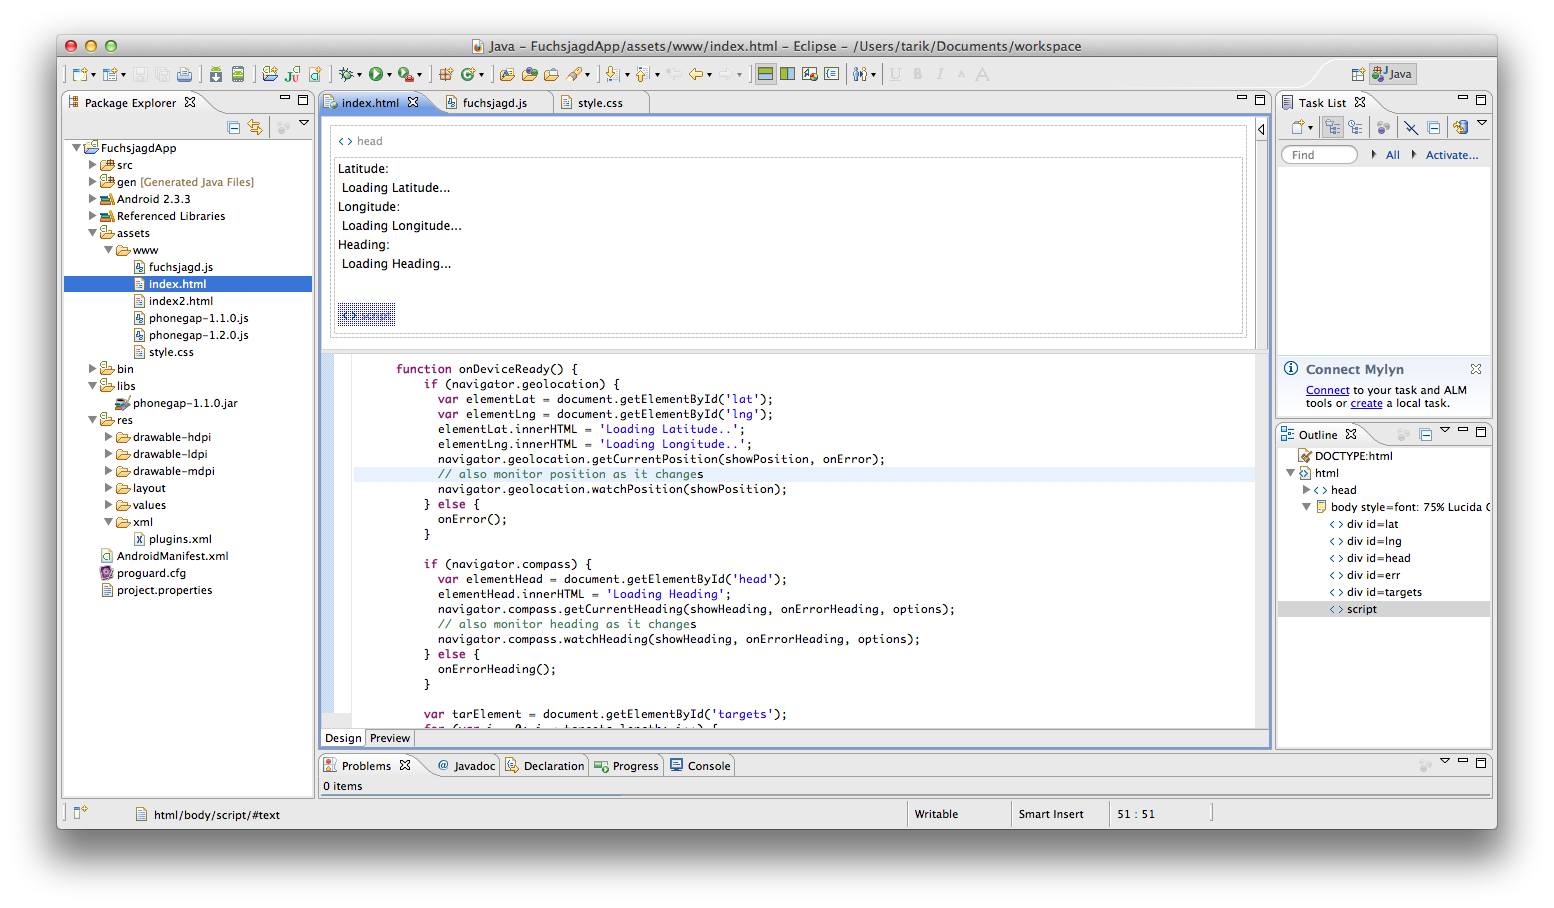
\includegraphics[width=14cm]{images/eclipse-shot.png}\\
		\caption{Entwicklungsumgebung Eclipse}
	\label{fig:eclipse-project}
\end{figure}

\subsubsection{Zugriff auf ein richtiges Android Phone} % (fold)
\label{ssub:Zugriff auf ein richtiges Android Phone}
Der Zugriff von Eclipse oder anderen IDEs auf ein Android Phone ist sehr einfach. Dazu muss lediglich in den Einstellungen auf dem Gerät unter Applikationen das Debug-Flag einschalten. Danach das Telefon mit dem USB Kabel an den Computer anhängen und beim laufen lassen einer Applikation erscheint es dann zur Auswahl in der Liste. Die Applikation wird dann deployed und installiert, und ist danach auch ohne Verbindung zum Computer verfügbar.
% subsubsection Zugriff auf ein richtiges Android Phone (end)

\subsubsection{Android Emulatoren} % (fold)
\label{ssub:Android Emulatoren}
Die Emulatoren, welche das Android SDK zu Verfügung stellt sind für einfache "`Hello World"' Appliktionen mehr als passable. Die Geschwindigkeit lässt jedoch schon beim Aufstarten von einem MacBook zu wünschen übrig. Der Angezeigte Android Desktop ruckelt und es dauert lange bis Klicks beantwortet werden. Wenn Andoid Native Features wie Geolocation oder der Kompass angesprochen werden sollen, muss dies zuerst kompliziert konfiugriert werden, wie es vielen Foren im Internet zu entnehmen ist. HTML5 und JavaScript funktionieren. Somit können die Emulatoren für einfache Regression Tests nützlich sein. Bei komplexeren Applikationen sollte man für das Programmieren jedoch ein richtiges Android Phone zur Verfügung haben wo man die Tests schnell und einfach darauf deployen und testen kann.
% subsubsection Android Emulatoren (end)

\subsubsection{Debuggen mit Eclipse} % (fold)
\label{ssub:Debuggen mit Eclipse}
Bei angehängtem Android Phone, können alle Aktivitäten im Eclipse angezeigt werden. Java Code könnte auch genau gedebugged werden. Leider können HTML und Java Script nicht gedebugged werden. Die Debug-View zeigt jedoch die Fehler wie einem Browser jedoch in chronologischem Ablauf zusammen mit den Warnings und Infos vom Phone (Klicks, Laden, etc). Somit kann dies dennoch hilfreich sein. 
% subsubsection Debuggen mit Eclipse (end)

\subsubsection{Probleme mit Android} % (fold)
\label{ssub:probleme_mit_android}
Initial hat der Setup eines einfachen PhoneGap "`Hello World"' Beispiels Schwierigkeiten bereiten, da es mit einer alternativen IDE versucht wurde. Für PhoneGap gibt es jedoch "`Getting-Started"'-Dokumentation nur mit Eclipse. Diese ist für jemanden, der noch nie mit Android SDK oder PhoneGap programmiert hat essentiell. \\
Weiter wurden die nativen Features Geolocation und vorallem Kompass lange einfach nicht angezeigt ohne eine Fehlermeldung zu liefern. Nach diversen "`Try and Error"' Versuchen mit Neuaufsetzten des Eclipse Android Projektes und sauberem Konfigurieren der eigentlich simplen Setup Schritten sind die Features dann gelaufen. 
% subsubsection Probleme mit Android (end)

% subsection Android (end)

\subsection{iPhone} % (fold)
\label{sub:iPhone}
iPhone Apps werden normalerweise in Xcode Programmiert. Phonegap gibt ein Xcode Projekt vor welches als Container für die eigentliche Applikation dient. Da man für die iPhone Entwicklung zwingend eine Apple Developer Lizenz benötigt, und damit die erstellten Applikationen signieren muss, kommt keine andere IDE in Frage. Die Projektansicht von Xcode ist auf Abbildung \ref{fig:xcode-project} zu sehen.

\begin{figure}[H]
	\centering			      
        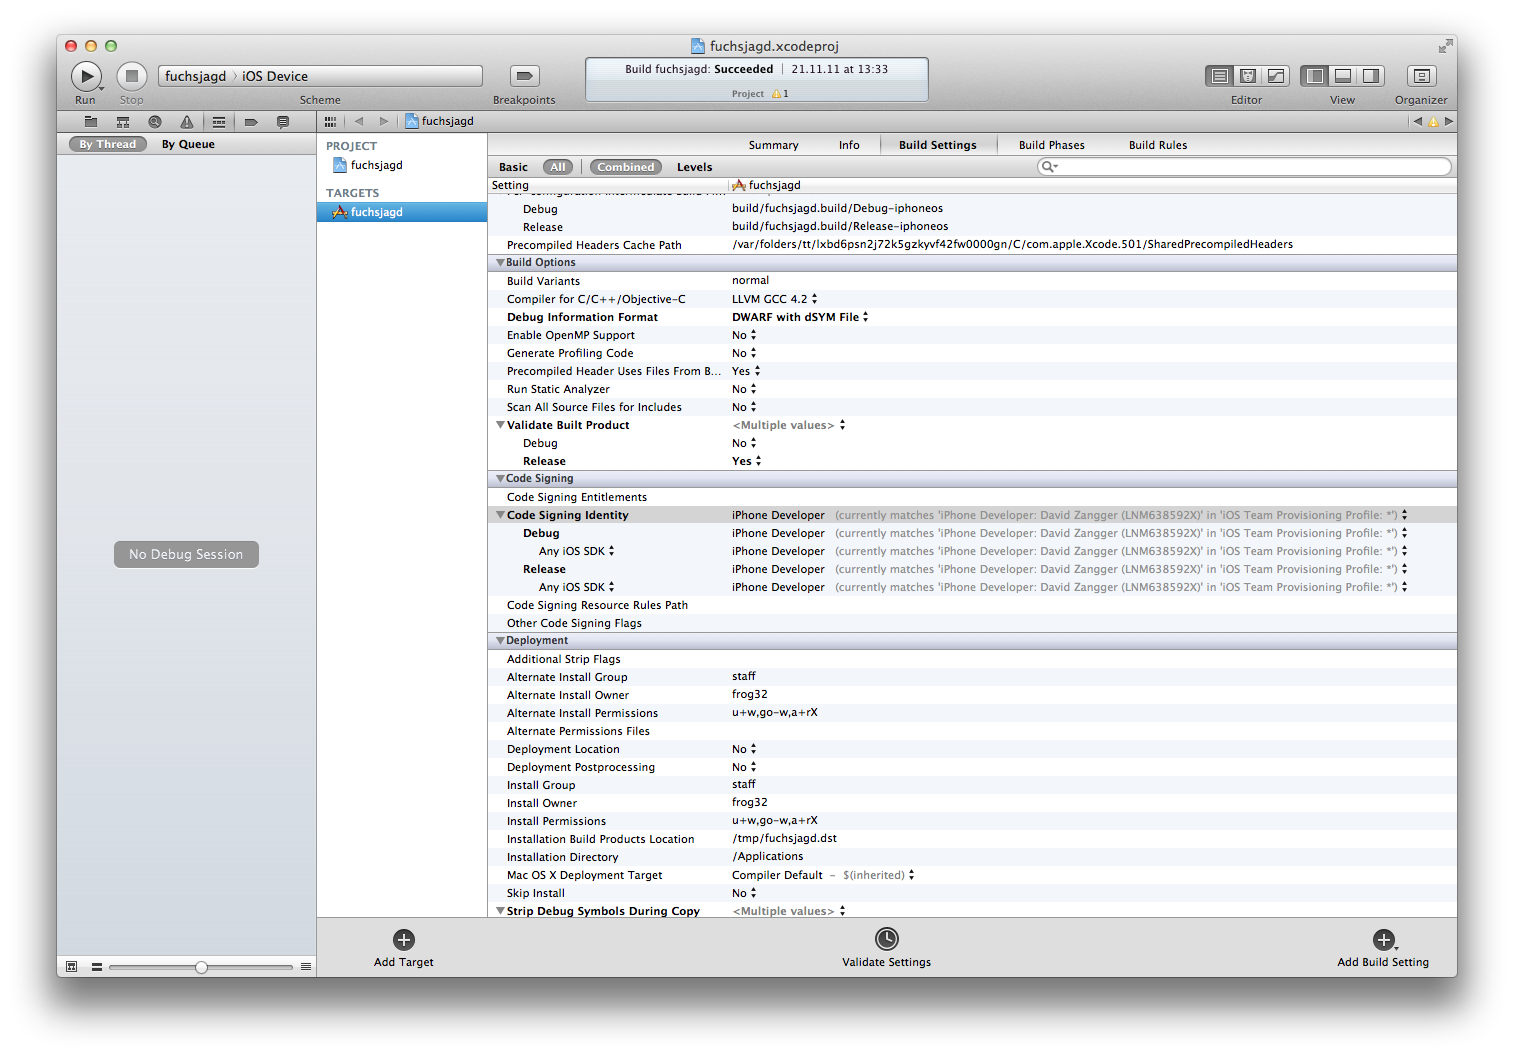
\includegraphics[width=14cm]{images/xcode-project.png}\\
		\caption{Entwicklungsumgebung Xcode}
	\label{fig:xcode-project}
\end{figure}

\subsubsection{Deployment auf ein iPhone} % (fold)
\label{ssub:Deployment auf ein iPhone}
Um eine eigen erstellte Applikation auf einem iPhone zu installieren, muss zuerst das iPhone zur Developer Lizenz hinzugefügt werden. Danach kann man über das Provisioning Portal von Xcode das iPhone zum aktuellen Projekt hinzufügen. Erst jetzt kann die Applikation mit den entsprechenden Signaturen kompilieret werden. Dieser Vorgang ist vor allem für Einsteiger ziemlich verwirrend und es lohnt sich hier eine gute Anleitung oder Hilfe eines erfahrenen Entwicklers zu holen.
% subsubsection Deployment auf ein iPhone (end)

\subsubsection{iPhone Emulator} % (fold)
\label{ssub:iPhone Emulator}
Das Ausprobieren der eigenen App auf einem Emulator ist mit Xcode ziemlich einfach. Man kann die iOS Version und den Gerätetyp über ein Menü auswählen, danach startet der Emulator und man kann die App Testen. Jedoch werden die Geolocation Services dann vom Entwicklungssystem übernommen, was dazu führt, dass die Ortung mittels WLAN Ortung funktioniert und dadurch sehr ungenau ist. Da Fuchsjagd stark auf Veränderungen der Geolocation angewiesen ist, kann die Kernfunktion nicht mit dem Emulator getestet werden.
% subsubsection iPhone Emulator (end)

\subsubsection{Debuggen von iPhone Apps} % (fold)
\label{ssub: Debuggen}
Der mitgelieferte Debugger welcher in Xcode enthalten ist, kann sowohl zusammen mit dem Emulator wie auch mit einem iPhone gebraucht werden und unterstützt viele nützliche Funktionen wie eine Messung des Speicherverbrauchs.
% subsubsection  Debuggen (end)

% subsection iPhone (end)
% section PhoneGap (end)
